%\documentclass[conference]{IEEEtran}
\documentclass[10pt,conference,anonymous]{IEEEtran}
\IEEEoverridecommandlockouts

%% Marcelo added this
\makeatletter
\renewcommand\footnoterule{%
  \kern-3\p@
  \hrule\@width.4\columnwidth
  \kern2.6\p@}
  \makeatother




\usepackage{inconsolata}
\usepackage{listings}

\lstset{language=Java,
basicstyle=\ttfamily\scriptsize,
%basicstyle=\ttfamily,
keywordstyle=\color{javapurple}\bfseries,
stringstyle=\color{pblue},
commentstyle=\color{javagreen},
morecomment=[s][\color{javadocblue}]{/**}{*/},
morecomment=[s][\color{gray}]{@}{\ },
numbers=left,
numberstyle=\tiny\color{black},
stepnumber=2,
numbersep=8pt,
tabsize=4,
showspaces=false,
showstringspaces=false,
breaklines=true,}

%%%%%%%%%%%%%%%%%%%%%%%%%%%%%%%%%%




\usepackage{adjustbox} % ajustar tabela ao tamanho da pagina

\usepackage{tikz}
\usetikzlibrary{matrix,fit,shapes,calc,positioning,shadows,arrows,shapes,backgrounds,decorations.markings,fadings}
\usepackage{graphicx}
\usepackage{multirow}
\usepackage[caption=false, font=footnotesize]{subfig}
\usepackage{wrapfig}
\usepackage{enumitem}
\usepackage{url}
%% helpers
\newcommand{\js}{JS}
\newcommand{\javascript}{JavaScript}
\newcommand{\es}{ES}
\newcommand{\ecmascript}{\es{}}
\newcommand{\tname}{TNAME}
\newcommand{\Comment}[1]{}
\newcommand{\numsubjects}{5}
\newcommand{\etal}{and colleagues'}
\newcommand{\ie}{i.e.}
\newcommand{\eg}{e.g.}
\newcommand{\cmark}{\ding{51}}%
\newcommand{\xmark}{{\color{red}\ding{55}}}%
\newcommand{\pGoodGood}{$\mathit{P}${\small\cmark\!\cmark}}%
\newcommand{\pGoodBad}{$\mathit{P}${\small\cmark\!\xmark}}%
\newcommand{\pBadDontCare}{$\mathit{P_?}$}%
\newcommand{\sfl}{SFL\xspace}
\newcommand{\ddg}{DDG\xspace}
\newcommand{\totfiles}{$\sim$38K}

%% annotations
\newif\ifdraftmode
%% Comment or uncomment the \draftmodetrue line.
\draftmodetrue
\ifdraftmode
 \newcommand{\Fix}[1]{\textbf{[[}{\color{red} #1}\textbf{]]}}
 \newcommand{\Mar}[1]{\textbf{[[Marcelo: }{\color{magenta} #1}\textbf{]]}}
 \newcommand{\Igor}[1]{\textbf{[[Igor: }{\color{blue} #1}\textbf{]]}}
 \newcommand{\note}[1]{\todo[inline,color=red!30,caption={}]{#1}}
\else
 \newcommand{\Fix}[1]{\relax}
 \newcommand{\Mar}[1]{\relax}
 \newcommand{\Igor}[1]{\relax}
 \newcommand{\note}[1]{\relax}
\fi

% For submitted version only.
\pagenumbering{arabic}

% Uncomment this if you need more space
%% \makeatletter
%% \def\@copyrightspace{\enlargethispage{-10pt}\relax}
%% \makeatother

\newcommand{\codesize}{\small}
\newcommand{\CodeIn}[1]{\mcodeid{#1}}
\newcommand{\CodeInM}[1]{\mcodeid{#1}}
% \|name| or \mathid{name} denotes identifiers and slots in formulas
\def\|#1|{\mathid{#1}}
\newcommand{\mathid}[1]{\ensuremath{\mathit{#1}}}
% \<name> or \codeid{name} denotes computer code identifiers
\def\<#1>{\codeid{#1}}
\newcommand{\codeid}[1]{\ifmmode{\mbox{\codesize\ttfamily{#1}}}\else{\codesize\ttfamily #1}\fi}
\def\<#1>{\mcodeid{#1}}
\newcommand{\mcodeid}[1]{\mbox{\codesize\ttfamily{#1}}}

%% thumbs up down
\newcommand*{\RightThumbsUpAux}[1]{%
  \begingroup
    \sbox0{Ag}%
    \raisebox{-\dp0}{%
      \includegraphics[{%
        height=\dimexpr\dp0+\ht0\relax,
        #1%
      }]{thumbsup.pdf}%
    }%
  \endgroup
}
\newcommand*{\RightThumbsUp}{%
  \RightThumbsUpAux{}%
}
\newcommand*{\RightThumbsDown}{%
  \RightThumbsUpAux{origin=c,angle=180}%
}
\newcommand*{\LeftThumbsUp}{%
  \scalebox{-1}[1]{\RightThumbsUp}%
}
\newcommand*{\LeftThumbsDown}{%
  \scalebox{-1}[1]{\RightThumbsDown}%
}

\newcommand{\checkm}{Y}
\newcommand{\crossmark}{N}
%\begin{wraptable}[20]{t}[0pt]{0.5\textwidth}

\newcommand{\totalTestFiles}{38,369}
\newcommand{\totalTestFilesCompileInAll}{35,939}
\newcommand{\totalTestFilesPassInAll}{24,493}
\newcommand{\nofuzzAll}{209}
\newcommand{\nofuzzBugs}{\Fix{XX}}
\newcommand{\nofuzzDuplicates}{63}
\newcommand{\nofuzzFalsePositives}{24}
\newcommand{\nofuzzHITotal}{177}
\newcommand{\nofuzzLOTotal}{32}
\newcommand{\nofuzzTotalFiles}{977} % conflicting files
\newcommand{\nofuzzFilesHI}{940} % conflicting files HI
\newcommand{\nofuzzFilesLO}{37} % conflicting files LO

\newcommand{\nofuzzBucketsBugsHI}{\Fix{124}} % buckets reported (including dups)
\newcommand{\nofuzzBucketsBugsLO}{\Fix{11}} % buckets reported
\newcommand{\nofuzzDupsHI}{\Fix{X}}
\newcommand{\nofuzzDupsLO}{\Fix{Y}}

% continue updating bugs table
\newcommand{\tableBugsNum}{\Fix{26}}

%% anonymize

\newcommand{\anonym}[1]{{\tiny\colorbox{black}{#1}}}

%% names
\newcommand{\radamsa}{radamsa}
\newcommand{\quickfuzz}{quickfuzz}

\newcommand{\jsc}{JavaScriptCore}
\newcommand{\veight}{V8}
\newcommand{\chakra}{Chakra}
\newcommand{\smonkey}{SpiderMonkey}
\newcommand{\jerry}{JerryScript}

\newcommand{\lo}{lo}
\newcommand{\hi}{hi}


\begin{document}

%Should I Fuzz my Inputs or Improve my Tests? 
\title{Leveraging Diversity to Find Bugs\\ in JavaScript Engines}

%% \author{
%% \IEEEauthorblockN{Sabrina Souto}
%% \IEEEauthorblockA{State University of Para\'iba\\
%% Para\'iba, Brazil\\
%% sabrinadfs@gmail.com}
%% \and
%% \IEEEauthorblockN{Marcelo d'Amorim}
%% \IEEEauthorblockA{Federal University of Pernambuco\\
%%   Pernambuco, Brazil\\
%%   damorim@cin.ufpe.br}
%% \and
%% \IEEEauthorblockN{Rohit Gheyi}
%% \IEEEauthorblockA{Federal University of Campina Grande\\
%%   Para\'iba, Brazil\\
%%   rohit@dsc.ufcg.edu.br}
%% }

\maketitle

%% page numbering -M
\thispagestyle{plain}
\pagestyle{plain}

%% JavaScript (\js{}) is a popular programming language for the
%% web. Finding errors in JS runtime engines is an important problem.
\begin{abstract}
JavaScript is a very popular programming language today. Checking
reliability of JavaScript engines is therefore an important
problem. This paper reports on a study to assess reliability of
JavaScript engines by leveraging the rich diversity of open-source
implementations. We explored two methods for that---test
transplantation and cross-engine differential testing. Test
transplatation evaluates the effects of running test suites of a given
engine in another engine. Cross-engine differential testing evaluates
the effects of fuzzing existing inputs and then comparing the output
produced by different engines with a differential oracle. Our results
indicate that \Fix{...}
\end{abstract}

\begin{IEEEkeywords}
JavaScript; Diversity; Software Testing
\end{IEEEkeywords}

\section{Introduction}

JavaScript (\js{}) is today one of the most popular programming
languages around~\cite{business-insider,stackify}, with significant
penetration in the segments of web development, mobile, and even for
client and server coding for the Internet of
Things~(IoT)~\cite{simply-technologies}.

The interest of the community for the language encourages constant
improvements in its specification and implementations.  It is natural
to expect that language improvements entails sensible implementation
changes. Even small changes can have high impact. For example, in
October 2014 a new attribute added to Array objects caused a bug that
resulted in the web app for the MS Outlook Calendar not working under
Chrome~\cite{array-bug-chromium-issue4247,array-bug-discussion}. Finding
bugs in JS engines is therefore an important problem given the range
of applications that could be affected. It is also challenging as
specifications evolve constantly and are incomplete. More
specifically, the evolution of the \js\ specification makes it hard to
assess if a test fails because of a bug or because of some missing
feature. The publicly-available Kangax compatibility
table~\cite{kangax} highlights this problem; it relates features with
the engines that (partially) support them. For similar reason, one
could misclassify a test failure as a bug when the failure could be,
in fact, caused by some undefined behavior in the spec. To note that
many of these cases exist as it can be observed by searching for
``implementation-dependent'' in the ES6 spec
document~\cite{ecmas262-spec}.

%% WHAT WE DID
This paper reports the results of a study we conducted to assess
reliability of existing JS engines by leveraging implementation
diversity in two orthogonal ways: test transplantation and
cross-engine differential testing.  \emph{Test transplantation}
evaluates the effects that running \js{} test files from a given
engine have in detecting bugs in other engines. The intuition is that
when a bug is found in some engine a test case is created and added to
the regression suite. Those test inputs often check interesting
scenarios that could reveal bugs in different engine
implementations. \emph{Cross-engine differential testing} evaluates
the bug-finding ability of fuzzing existing
inputs~\cite{fuzz-testing-history} and then comparing the output
produced by different engines using a differential oracle. One of
various causes of output discrepancy is a bug. It is worth noting that
Differential Testing~\cite{Brumley-etal-ss07} (DT) has been applied in
a variety of contexts to find
bugs~\cite{Yang-etal-pldi11,Chen-etal-fse2015,Argyros-etla-ccs16,Chen-etal-pldi16,petsios-etal-sp2017,SivakornAPKJ17,Zhang:2017:ATD:3097368.3097448}. It
automates test generation in scenarios where multiple implementations
of a system exist. DT leverages the diversity across system's
implementations to detect anomalous behavior. For example, Mozilla
runs JS files--created with the grammar-based fuzzer
jsfunfuzz~\cite{jsfunfuzz}--against different configurations of their
SpiderMonkey engine~\cite{jsfunfuzz-mozilla-bug} to find discrepancies
across different configurations of the same build (\eg{}, enabling or
not eager JIT compilation). They use this technique since 2002 and
have been able to find over 270 bugs since
then~\cite{jsfunfuzz-at-mozilla}, including security bugs.  In
contrast, cross-engine differential testing--the technique used in
this work--checks functional correctness by comparing the output
produced by \emph{different engines} on a fuzzed
input~\cite{patra2016learning}. This approach has not been
popularized, certainly because it is impractical to fully automate--a
number of legitimate reasons exist, other than a bug, for a test
execution to manifest discrepancy (see
Table~\ref{tab:false-positives}). This study quantifies human effort
to find these bugs using this method.

%% WHAT WE FOUND
To sum, we found that \Fix{...}

%% LIST OF CONTRIBUTIONS
This paper makes the following contributions \Fix{...}

\section{JavaScript}
\label{sec:es6-design}
\label{sec:imp-dep-behavior}

JavaScript engines are virtual machines that parse source code,
compile it in bytecodes, and run these bytecodes. These engines
implement some version of the ECMAScript (\es{}), which emerged with
the goal to standardize variants of the language, such as Netscape's
JavaScript and Microsoft's JScript\footnote{The name JavaScript still
  prevails today, certainly for historical reasons.}. The \es{}
specification is regulated by Ecma International~\cite{es6-website}
under the TC39~\cite{tc39-github} technical committee.  Every year, a
new version of the \es{} specification is produced with new features
and minor fixes. The canonical spec today is
ES6~\cite{ecmas262-spec-repo,ecmas262-spec}.

%% In the following, we briefly describe different sources of
%% discrepancies that can emerge across different engine implementations
%% as results of the active changes in the \es{} specification.
%% .........
%% A compatibility table relating features and supporting engines is
%% publicly available~\cite{kangax}.

Both the specification and implementation of JavaScript are
incomplete. Certain parts of the specification are undefined; it is
responsibility of engine engineers to decide how to implement these
functionalities. The JavaScript spec uses the label
``implementation-dependent'' to indicate these cases, where behavior
may differ from engine to engine. One reason this flexibility in the
spec exists is to enable compiler optimizations. For example, the
\mcodeid{for-in} loop does not clearly specify the iteration
order~\cite{so-forin-undefined,javascript-in-chrome} and different
engines capitalize on that~\cite{for-in-undefined}.  As another
example, the latest version of the \es{} specification states that if
the \mcodeid{Number.toPrecision()} function is called with more than
one argument, then the behavior is
implementation-dependent~\cite{es6-toPrecision}. Various other cases
like these exist in the specification. Such gap also exists at the
implementation level. Given the speed the specification changes and
the complexity of the language some features are not fully implemented
as can be observed by the Kangax compatibility table~\cite{kangax}.

\sloppy It is also worth noting that, as in other languages, some
elements in JS have non-deterministic behavior (\eg{},
\mcodeid{Math.random} and \mcodeid{Date}). A test that make decisions
based on these elements could, in principle, produce different
outcomes on different runs. Carefully-written test cases should not
manifest this kind of
flakiness~\cite{luo-etal-fse2014,palomba-zaidman-icsme2017}, but
fuzzed test files could are more likely, intuitively, to manifest
them.

As mentioned previously, all those aspects make testing \js\ engines
more challenging.


%\subsection{Randomness}


%\subsection{\Fix{Other}}

%% 1) The stack depth in JS is often close to the real (native) C stack
%% depth, nevertheless observable by JS through recursion. This causes
%% differential behavior even on the same engine when JITs are enabled or
%% disabled, as the stack frame sizes vary. LangFuzz in particular
%% produces a lot of recursions and hits these problems even more often
%% than jsfunfuzz.\Mar{ask C. Holler. it is unclear to me how the output
%%   could be different.}


\section{Differential Testing Infrastructure}
\label{sec:design}


Figure~\ref{fig:workflow} illustrates the infrastructure we used for
differential testing, use in part of our study. The bug-finding
process takes on input JS files from regression test suites of various
JS engines and generates warnings on output. Boxes in the figure
denote encapsulation; arrowed lines indicate data flow. The cycle
icons denote repetition--the leftmost icon indicates that each file in
the input list will be analyzed in separate whereas the rightmost icon
shows that a single file will be fuzzed multiple times.

%\begin{wrapfigure}[10]{r}[0pt]{0.45\textwidth}
\begin{figure}[h]
  \centering
%  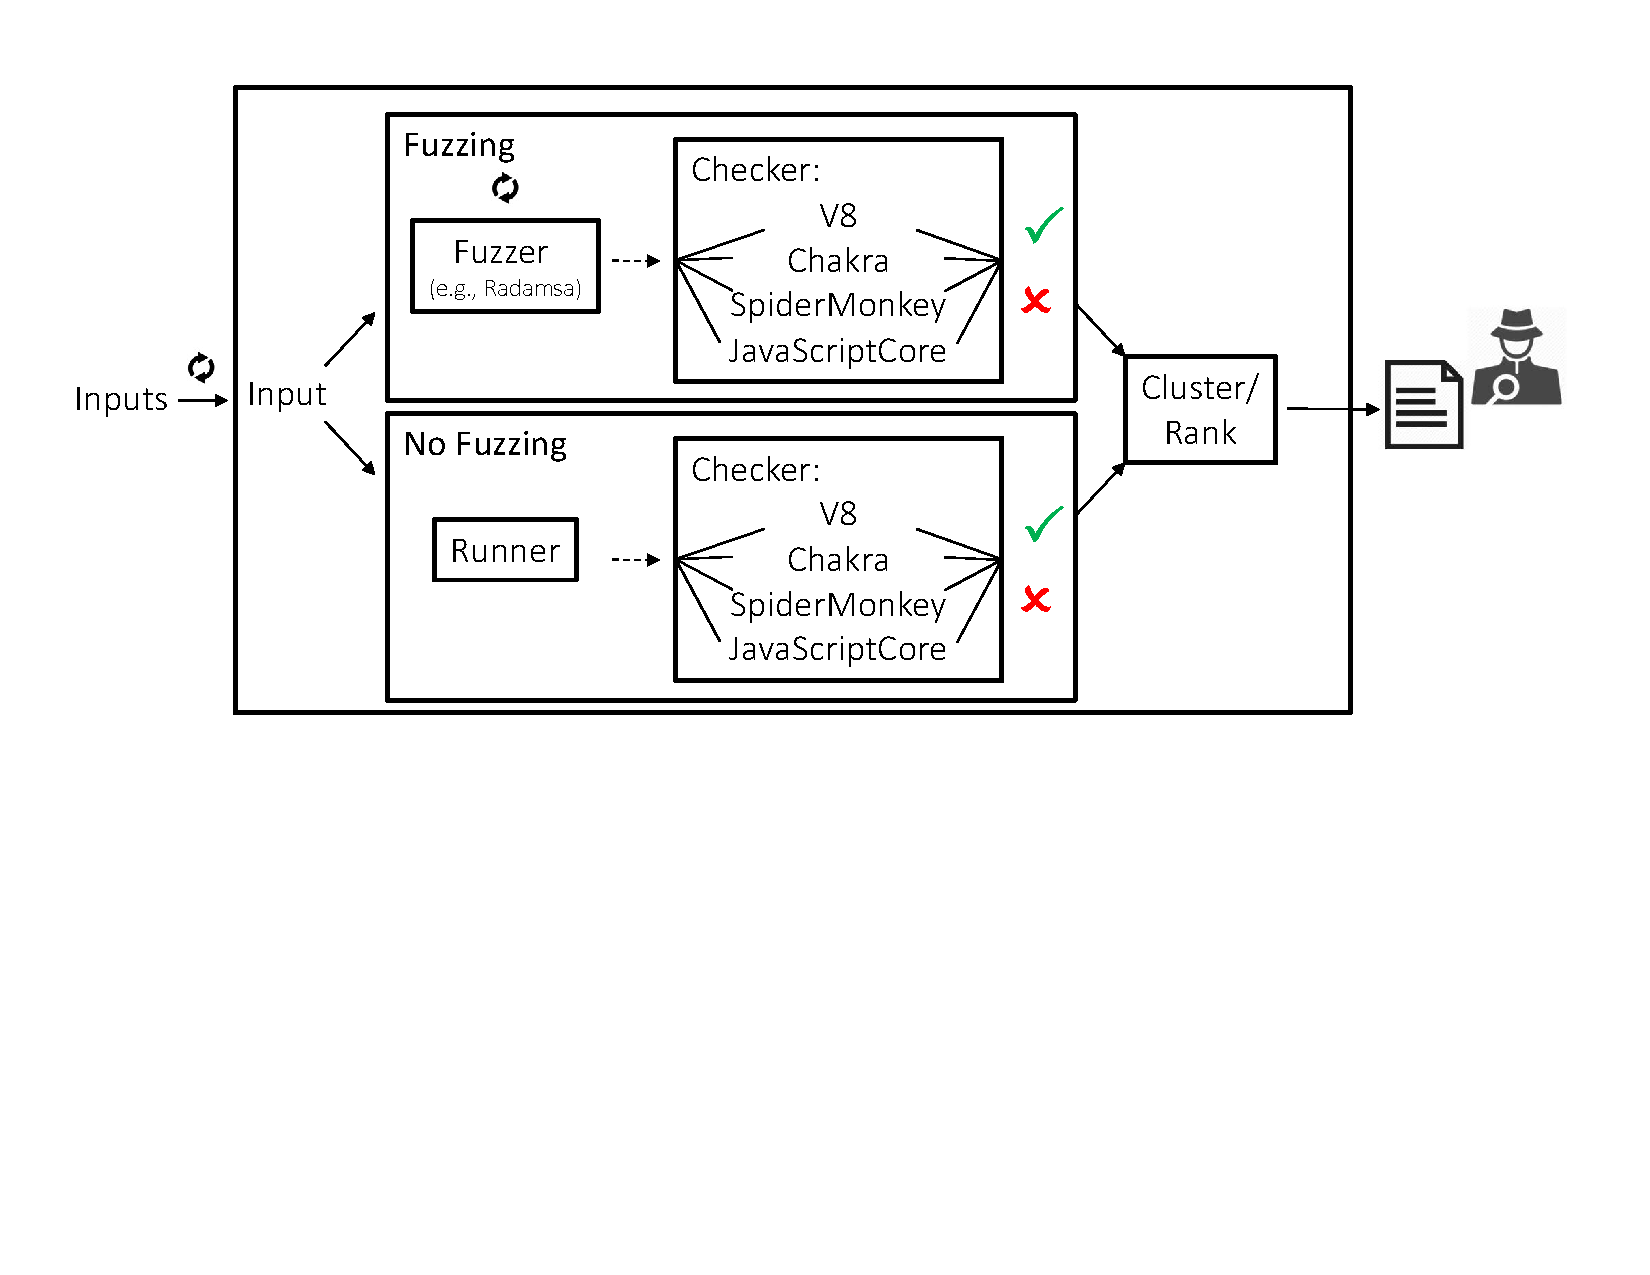
\includegraphics[trim=20 350 200
%    0,clip,width=0.35\textwidth]{google-awards-workflow}
  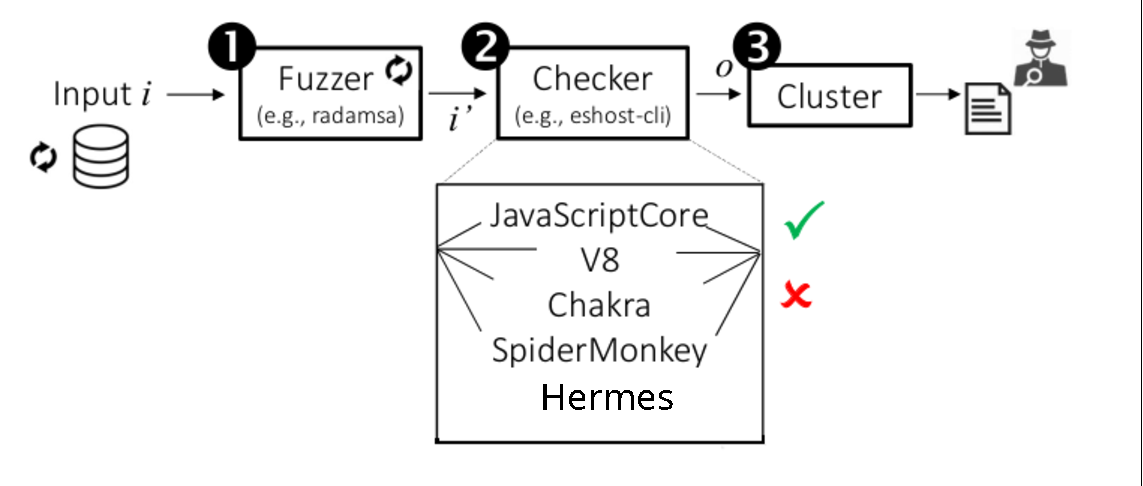
\includegraphics[trim=0 350 0 0,clip,width=0.65\textwidth]{diff-testing-runtimes}
  \caption{\label{fig:workflow}Differential Testing infrastructure overview.}
\end{figure}

The bug-finding process works as follows. New inputs are obtained for
a given test input using some off-the-shelf input
fuzzer~\cite{fuzz-testing-history}.\Comment{ Several fuzzing methods
  have been proposed in the past, varying with respect to how new
  inputs are
  generated~\cite{afl,honggfuzz,grammarinator,jsfunfuzz,radamsa}.}
Section~\ref{sec:objects:fuzzers} describes the fuzzers we selected.
The oracle checks whether or not the output produced for the fuzzed
file is consistent across all engines. In case the test passes in all
engines or fails in all engines (\ie{}, the output is consistent), the
infrastructure discards the test. Otherwise, it considers the input as
potentially fault-revealing; hence interesting for human
inspection. Note that a number of reasons exist, other than a bug, to
explain discrepancy (see Table~\ref{tab:false-positives}). We used the
open-source eshost-cli project~\cite{eshost-cli}, also used at
Microsoft, for checking output discrepancy.

%The checker can produce multiple warnings for a given input. 

Recall that a warning can be manifested for reasons other than a bug
and there is no clear way to distiguish those cases automatically (see
Table~\ref{tab:false-positives}). A human needs to inspect the warning
to diagnose the discrepancy. To facilitate inspection, the
infrastructure prioritize these warnings and clusters them in
groups. Considering prioritization, we classified warnings in two
kinds, reflecting their likelihood to manifest a real bug. Warnings of
the kind ``\hi{}'' are associated with the cases where the test code
executed to completion without violating any internal checks but it
violated assertions declared in the test itself or its harness. The
rationale is that the input is valid--considering the checks declared
in the API functions--but, still, it manifests discrepancy through
violation of an assertion declared in the test.\Mar{example!} In constrast, warnings
in the ``\lo{}'' group reflect the cases where the anomaly was
observed during the execution of functions not related to the test
itself. We found that different engines often check pre-conditions of
those functions differently. It can happen, for example, that one
engine enforces a weaker pre-condition on a function input compared to
another engine and that is acceptable.\Mar{example!} In those cases, our infrastructure would
observe a discrepancy that is more likely to be associated with an
invalid input produced by the fuzzer, \ie{}, it is likely to be a bug
in the test code not the engine (library or runtime) code. Although we
did find real bugs from ``\lo{}'' warnings, the proportion was much
lower compared to ``\hi{}'' warnings. Overall, only \Fix{12\%} of the
reals bugs we found originated from ``\lo{}'' warnings.

\Mar{explain what is a bucket (we refer to it later).} 

\section{Objects of Study}
\label{sec:methodology}

This section discusses the objects we used in our study.

\subsection{Engines}
\label{sec:methodology:engines}~We selected 
JS engines according to the following criteria.

\begin{itemize}
\item Released latest version after Jan 1, 2018
\item Contains more than 1K starts, if on GitHub  
\item Uses a public issue tracker
\end{itemize}  

We look for highly-maintained (as per the first criterion) and popular
(as per the second criterion) projects. As we wanted to report bugs,
we also looked for project with public issue
trackers. Table~\ref{tab:engines} lists the engines we analyzed in
this work. It is worth noting that we used GoogleChromeLab's JSVU
tool~\cite{jsvu} to automatically install and configure versions of
different JS engines in our host environment. This is important as we
aim to use the most recent stable versions of each engine as to avoid
reporting old and already-fixed bugs to developers.

%% Table~\ref{tab:engines} shows the engines we selected in this
%% study. We made an exception to the second criterion with
%% XS~\cite{xs2018repo}. As the project is young, created in Oct 2017, we
%% thought there was insufficient time to obtain 1K stars for XS. We
%% still considered this project as it seems to be attracting interest
%% from the community\Fix{is this true?}

\begin{table}[t]
  \centering
  \caption{\label{tab:engines}Engines Analyzed.}
  \begin{tabular}{cccr}
    \toprule
    Team & Name & URL & \# Stars \\
    \midrule
    Apple & \jsc{} (WebKit) & \cite{jsc2018repo} & \multicolumn{1}{c}{3300+} \\
    Google & \veight{} & \cite{v82018repo} & 9800+ \\
%    JerryScript & JerryScript & \cite{jerryscript2018repo} & 3100+ \\
    Microsoft & \chakra{} & \cite{chakra2018repo} & 7200+ \\
%    Moddable & XS & \cite{xs2018repo} & 140+ \\
    %% \midrule
    %% \multirow{2}{*}{Mozilla} & Rhino & \cite{rhino2018repo} & 1800+ \\
    Mozilla & \smonkey{} & \cite{spidermonkey2018repo} & \multicolumn{1}{c}{1100+} \\
   \bottomrule     
  \end{tabular}
\end{table}

\subsection{Seed JS files\label{sec:seeds}}~
We selected test files from several public projects from GitHub. We
looked for self-contained tests from JS engine projects, initially
using the GitHub REST API~\cite{github-rest-api}. We noticed that some
of the tests we found depend on external libraries, which not all
engines we use support. We decided to discard those. For example, many
tests we found required a Node.js runtime~\cite{node} for
execution. The main source of test cases is the offical
Test262~\cite{tc39-github} conformance test suite for the ECMA262
specification~\cite{ecmas262-spec}. This test suite contains 87\% of
all the tests we used. We also considered test suites of three of the
four engines mentioned in Section~\ref{sec:methodology:engines} and
four other engines. Table~\ref{tab:test-suites} shows the breakdown of
tests we considered. Overall, we found a total of \totfiles{} JS
files. We did not consider tests from the \chakra{} repository because
they depend on non-portable objects. Notice that the number of tests
in \veight\ is low. That happens because many tests in \veight{} are
inherited from Mozilla and \jsc{}; we discarded those to avoid
repetition and to give credit where it is due. The \veight{} test
suite contains other tests, but, as in \chakra{}, these tests use
non-portable testing objects that we still did not mock.

It is also worth mentioning that some engines use a custom shell to
run tests, including a harness with specific assertions.  For these,
we needed to make small changes in the testing infrastructure to be
able to run the tests uniformly across all engines. More precisely, we
needed to mock non-portable harness functions, which are only
available to certain engines.

\begin{table}[t]
  \centering
  \caption{\label{tab:test-suites}Test Suites. The sections of the
    table show, respectively, the TC-39 conformance test suite, suites
    from engines we analyzed, and suites from other engines.}
  \begin{tabular}{ccr}
    \toprule
    Name & Source & \# JS files \\
    \midrule
    TC-39 (Test262) & \cite{ecma262-conformance-suite} & 31,276 \\
    \midrule
    Mozilla & \cite{mozilla} & 2,633 \\
    \veight{} & \cite{v8} & 74 \\
    \jsc{} & \cite{webkit} & 1,031 \\
    \midrule    
    Duktape & \cite{duktape} & 1,195 \\ 
    JerryScript & \cite{jerryscript} & 1,950 \\
    JSI & \cite{jsi} & 98 \\
    Tiny-js & \cite{tinyjs} & 48 \\    
    % Chakra & \cite{chakracore} & 2632 \\
    \midrule
     &  & \totalTestFiles{} \\
   \bottomrule     
  \end{tabular}
\end{table}

% For example to run the JerryScript tests it was necessary 
% use the unit-test package to run it, but with our changes we added the assertion
% does not have an assertion in the test file
% \Fix{add code to explain}

\subsection{Fuzzers}
\label{sec:objects:fuzzers}

%% In the following, we describe the list of fuzzers we analyzed. We
%% initially considered generational grammar-based fuzzers and mutational
%% fuzzers.

Fuzzers are typically categorized in two main groups--those that build
inputs anew (generational) and those that modify existing inputs
(mutational). We used two black-box mutational
fuzzers\Comment{Radamsa~\cite{radamsa} and QuickFuzz~\cite{quickfuzz}}
in this study. In the following, we provide rationale for this
selection.

Generational fuzzers are typically grammar-based. These fuzzers
generate a new file using the grammar of the language whose inputs
should be fuzzed. Intuitively, those fuzzers implement a traversal of
the production rules of the input grammar to create syntax trees,
which are then pretty-printed. Consequently, this approach produces
inputs that are syntactically valid by construction. We analyzed four
grammar-based fuzzers--Grammarinator~\cite{grammarinator},
jsfunfuzz~\cite{jsfunfuzz},
LangFuzz~\cite{Holler:2012:FCF:2362793.2362831}, and
Megadeth~\cite{grieco2016quickfuzz}.  Unfortunately, none of those
were effective out of the box. For example, we produced 100K inputs
with Grammarinator and only \Fix{X} of those were valid. With
Megadeth, we were able to produce \Fix{Y, Y$>$Y?}  valid inputs as it
contains some heuristics to circumvent violations of certain type
rules such as \Fix{variable used must be defined?}. Nonetheless,
running those inputs in our infrastructure we were unable to find
discrepancies. Inpecting those inputs, we realized that they reflected
very simple scenarios. To sum, a high percentage of inputs that
Grammarinator and Megadeth generated were semantically-invalid that we
needed to discard whereas the valid inputs manifested no
discrepancies. Considering jsfunfuzz~\cite{jsfunfuzz}, we noticed
that, in addition to the issues mentioned above, it produces inputs
that use functions that are only available in the SpiderMonkey
engine. We would need either to mock those functions in other engines
or to discard those tests. Considering
LangFuzz~\cite{Holler:2012:FCF:2362793.2362831}, the tool is not
publicly available. One fundamental issue associated with generational
fuzzers in our context is that the tests they produce do not contain
assertions; to enable the integration of this kind of fuzzers in our
infrastructure, we would need to look for discrepancies across
compiler messages.  All in all, although grammar-based fuzzers have
been shown effective to find real
bugs~\cite{Holler:2012:FCF:2362793.2362831}, generating valid inputs,
albeit promising conceptually, still requires some engineering
effort. For this reason, we did not consider those fuzzers in this
study.

%% Our
%% infrastructure supports any grammar fuzzer with a few
%% adjusts. However, we try to integrate several grammar-based fuzzers,
%% for example
%% and \Fix{others fuzzers} to
%% generate new JavaScript files based on grammar, but after several runs
%% it was observed that this approach was ineffective due the amount of
%% invalid files and/or files without discrepancies.
%% For example, if we
%% ran Grammarinator to generate 1K JS files ten times with a random seed
%% generation, we obtained \Fix{XX\%} of valid files. Checking in our
%% environment almost \Fix{XX\%} are js files that shows undefined
%% variables and due the differential testing in our environment all
%% engines will raise a SyntaxError and this approach was not relevant to
%% our experiment.

%% We initially considered used representatives of popular fuzzing approaches. For
%% random-based fuzzing we used Radamsa~\cite{radamsa}; for
%% coverage-based fuzzing we used
%% \Fix{AFL~\cite{afl}/libfuzzer~\cite{libfuzzer}?}, and for
%% generative-based fuzzing we used
%% \Fix{grammarinator,jsfunfuzz?}. Details on how these fuzzers work can
%% be found elsewhere~\cite{fuzz-bart}.

Mutational fuzzers can be either white-box or black-box. White-box
mutational fuzzers are typically coverage-based. American Fuzz Loop
(AFL)~\cite{afl} and libFuzzer~\cite{libfuzzer} are examples of this
kind of fuzzers. These fuzzers run tests inputs against instrumented
versions of the program under testing with the typical goal of finding
univeral errors like crashes and buffer overflows. The instrumentation
adds code to collect branch coverage and to monitor specific
properties\footnote{There are options in the clang toolchain to build
  programs with fuzzing instrumentation~\cite{libfuzzer}. clang
  provides several sanitizers for property
  checking~\cite{clang-documentation}.}. AFL use coverage to determine
inputs that uncover a new branch and hence should be fuzzed more
whereas libFuzzer uses evolutionary generation--it tries to minimize
the distances to still-uncovered branches of the program. AFL takes
the instrumented program binary (say, a JS engine) and one seed input
to that program (say, a JS program) and produces on output
fault-revealing inputs, if found. Considering our context of
application, we needed to instrument one runtime engine for fuzzing;
we chose v8. Unfortunately, we found that most of the inputs produced
by AFL violate the JS grammar. Furthermore, the fuzzing task can take
days for a single seed input and there is no simple way to guide the
exploration\footnote{Exchanged emails with the tool author.}. That
happens because the fuzzer aims to explore the entire decision tree
induced from the engine's main function, including the branches
associated with the higher layers of the compiler (\eg{}, lexer and
parser). It is worth mentioning that Google mitigates that problem
with libFuzzer by asking developers to create fuzz targets for
specific program
functions\cite{libFuzzer-tutorial-google,libFuzzer-chromium-google}. Although
that approach has shown very effective, it requires domain knowledge
to create the calling context to invoke the fuzz target. For those
reasons, coverage-based fuzzers were not considered in this study.

We used two black-box mutational fuzzers in this
study--\radamsa~\cite{radamsa} and \quickfuzz~\cite{quickfuzz}. These
fuzzers require no instrumentation and domain-knowledge. They mutate
\emph{existing} inputs randomly. The strenght of the approach is
limited by the quality of the test suite and the supported mutation
operators, which are typically simple. We chose \radamsa\ and
\quickfuzz\ \Fix{...elaborate...} \Mar{I mention below that these
  fuzzers ``only make valid changes in literals of the
  language''. Please confirm and explain that still this is
  interesting!}


\section{Results}
\label{sec:results}

The goal of our study is to assess reliability of \js\ engines by
leveraging implementation diversity, which is specially rich in this
domain. We report results in three parts. First, we report on the
stability of the engines we analyzed using the Test262 standard
conformance test suite for EcmaScript~\cite{ecma262-conformance-suite}
(Section~\ref{sec:stability}). The intuition is that the bugs we
discover throughout this study would have low relevance if the engines
are too fragile. Second, we report results obtained with test
transplantation (Section~\ref{sec:transplantation}). The rationale is
that the domain of possible inputs is too large; consequently, we
expect that test suites written for a given engine cover scenarios and
corner cases uncovered by another engine. To sum, we hope that that
test cases written for one engine could reveal bugs in different
engines as opposed to only manifesting false alarms such as those that
could emerge from implementation-dependent behavior. Third, we
analyzed the impact of using cross-engine differential testing to find
bugs (Section~\ref{sec:cross-engine-diff-testing-results}). The
rationale is that even black-box fuzzers that typicaly make valid
changes only in literals of the language could expose important
bugs. All in all, we want to assess the impact of simple approaches
that leverage on diversity to find bugs in \js\ engines with the goal
of assessing their reliability.

\subsection{Stability of Engines}
\label{sec:stability}

We evaluated stability with Test262~\cite{ecma262-conformance-suite},
the official \js{} conformance test suite for the ECMA262
specification. We ran this suite once a day for seven consecutive
days. Table~\ref{tab:test262} shows the number of failures over this
period. It is important to note that failures are expected as it takes
time for engines to adjust to the spec. It is also important to
highlight that all engines we analyzed, but \chakra{}, use some
variant of the Test262 suite as part of their regression
process\Mar{with fewer tests?}. We used the official version
instead\Mar{, which updates tests regularly?}. To sum, we observed
that \Fix{...} \Mar{justify regressions using the kangax report}

\begin{table}[h]
  \centering
  \caption{\label{tab:test262}Number of failures in Test262 over
    a 7-day period.}
  \begin{tabular}{crrrrrrr}
    \toprule
    engine\textbackslash{}day& 1 & 2 & 3 & 4 & 5 & 6 & 7 \\
    \midrule
    \jsc{} & - & - & - & - & - & - & - \\
    \veight{} & - & - & - & - & - & - & - \\
    \chakra{} & - & - & - & - & - & - & - \\
    \smonkey{} & - & - & - & - & - & - & - \\
    \bottomrule 
  \end{tabular}
\end{table}



\subsection{Test Transplantation}
\label{sec:transplantation}

This section reports results obtained with test
transplantation. Table~\ref{tab:cross-testing} shows the number of
failures that each engine produces on a different test suite. To sum,
we observed that \Fix{...}

\begin{table}[h]
  \centering
  \caption{\label{tab:cross-testing}Number of failures observed exchanging
  test suites.}
  \begin{tabular}{crrrr}
    \toprule
    test suite\textbackslash{}engine & \jsc{} & \veight{} & \smonkey{} & \chakra{}\\
    \midrule
    \Fix{Versions (01.08)} & 234485 & 7.0.126 & 62.0b13 & 1.10.1 \\
    \midrule
    \jsc{} & \Fix{10} & 11 & 107 & 157   \\
    \veight{} & 29 & \Fix{0} & 0 & 0  \\
%    \chakra{} & - & - & - & -  \\
    Mozilla & 741 & 286 & \Fix{178} & 476   \\
    Duktape & 238 & 80 & 202 & 85   \\
    JerryScript & 94 & 89 & 90 & 91   \\
    JSI & 35 & 14 & 14 & 14   \\
    Tiny-js & 11 & 11 & 11 & 11  \\
    \bottomrule 
  \end{tabular}
\end{table}  

%% Our infrastructure reported a total of \nofuzzAll{} buckets, including
%% \lo{} and \hi{}, that resulted in \nofuzzBugs{} bug reports. Of the
%% total of \nofuzzAll{} buckets, we found that \nofuzzDuplicates\ were
%% duplicates and \nofuzzFalsePositives\ were false positives. Most of
%% the cases of duplicates were related to the Test262 conformance test
%% suite, which all \js{} should strive to pass but we found that it is
%% not uncommon for the engines to fail on some of these. For example,
%% \veight{} \nofuzzFalsePositives

We inspected each of those failures in detail according to the
following methodology. \Fix{..elaborate..}
Figure~\ref{tab:test-transplantation-bugs} shows
results. \Fix{...elaborate...}

\begin{table*}[t]
  \vspace{-3ex}
%  \scriptsize
  \centering
  \caption{List of bug reports issued as result of test transplantation.}
  \label{tab:test-transplantation-bugs}
  \begin{tabular}{cccccccc}
    \toprule Issue\#    & Date & Fuzz & Engine  & Status  & \multicolumn{1}{c}{Url}  & Severity & Suite \\
    \midrule    
    1  & 4/18 & \crossmark & JavascriptCore  & New  & \anonym{\href{https://bugs.webkit.org/show\_bug.cgi?id=184749}{\#184749}} & \Fix{x} & JerryScript      \\
   2  & 4/23 & \crossmark & Chakra  & \textbf{Confirmed}  & \anonym{\href{https://github.com/Microsoft/ChakraCore/issues/5033}{\#5033}} & \Fix{x} & Mozilla      \\
   3  & 4/29 & \crossmark & Chakra  & \textbf{Confirmed}   &
    \anonym{\href{https://github.com/Microsoft/ChakraCore/issues/5065}{\#5065}} & \Fix{x} & Mozilla \\
   \multirow{2}{*}{4}  & \multirow{2}{*}{4/29} &  \multirow{2}{*}{\crossmark} & Chakra & \textbf{Confirmed} &    \anonym{\href{https://github.com/Microsoft/ChakraCore/issues/5067}{\#5067}} & \multirow{2}{*}{\Fix{x}} & \multirow{2}{*}{Mozilla}\\
                       &  &                       &
    JavascriptCore & New &    \anonym{\href{https://bugs.webkit.org/show\_bug.cgi?id=185130}{\#185130} } &   & \\
   5 & 5/02 & \crossmark & JavascriptCore & New  & \anonym{\href{https://bugs.webkit.org/show\_bug.cgi?id=185208}{\#185208}} & \Fix{x} & Mozilla \\
   6 & 5/17 & \crossmark & Chakra & \textbf{Confirmed} & \anonym{\href{https://github.com/Microsoft/ChakraCore/issues/5187}{\#5187}} & \Fix{x} & \jsc{}\\
   7 & 5/21 & \crossmark & Chakra & \textbf{Confirmed} & \anonym{\href{https://github.com/Microsoft/ChakraCore/issues/5203}{\#5203}} & \Fix{x} & Mozilla\\
   8 & 6/28 & \crossmark & Chakra & \textbf{Confirmed}  & \anonym{\href{https://github.com/Microsoft/ChakraCore/issues/5388}{\#5388}} & \Fix{x} & \jsc{}\\
   9 & 7/10 & \crossmark & Chakra & \textbf{Confirmed} & \anonym{\href{https://github.com/Microsoft/ChakraCore/issues/5442}{\#5442}} & \Fix{x} & JerryScript\\
  10 & 7/18 & \crossmark & Chakra & \textbf{Fixed} & \anonym{\href{https://github.com/Microsoft/ChakraCore/issues/5478}{\#5478}} & \Fix{x} & Mozilla\\
   11 & 7/18 & \crossmark & JavascriptCore & New & \anonym{\href{https://bugs.webkit.org/show_bug.cgi?id=187777}{\#187777}} & \Fix{x} & JerryScript\\
   \bottomrule
  \end{tabular}
\end{table*}


\subsection{Cross-Engine Differential Testing}
\label{sec:cross-engine-diff-testing-results}

\begin{figure}[t]
  \centering
  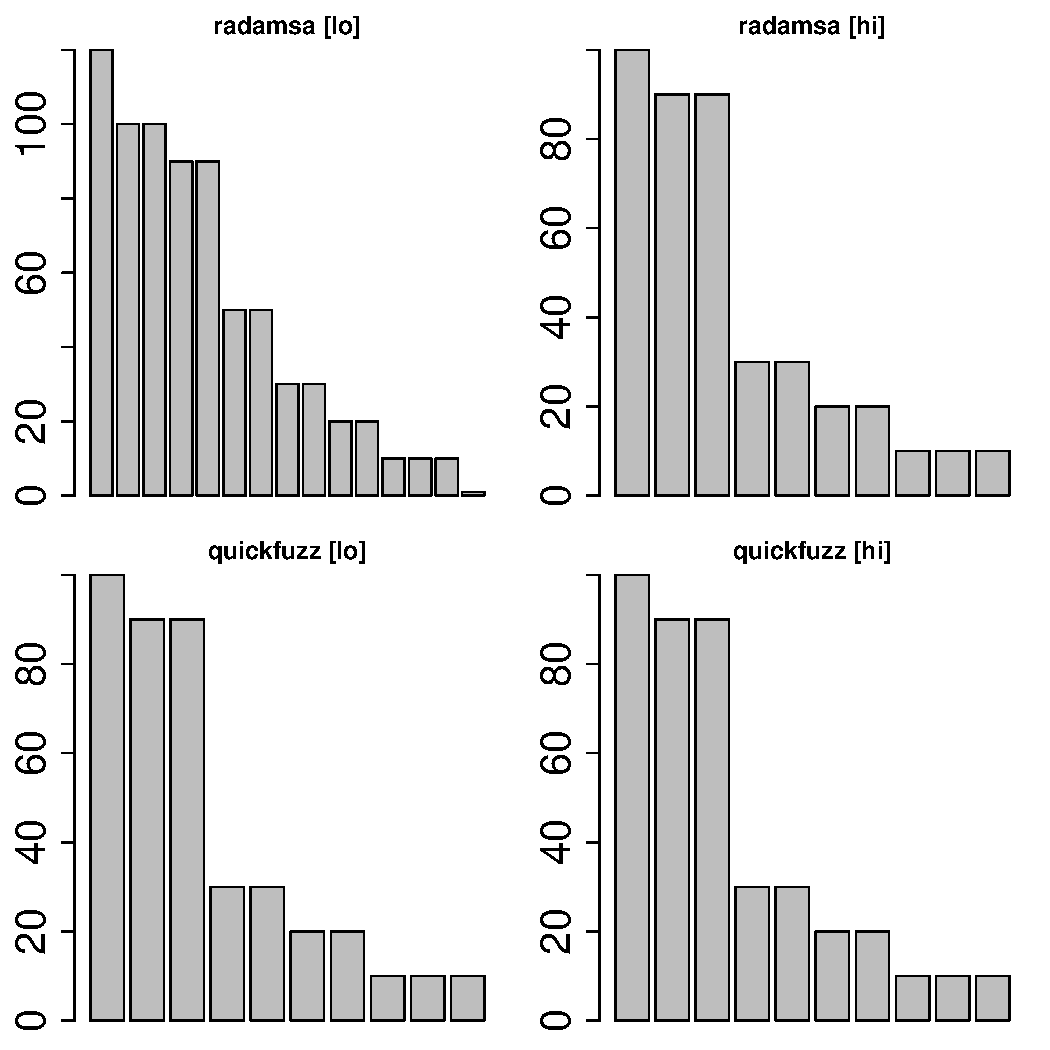
\includegraphics[trim=0 0 0 0,clip,width=0.40\textwidth]{R/histograms/histograms.pdf}  
  \caption{\label{fig:distribution}Distribution of lo and hi warnings
   in buckets.}
\end{figure}

This section reports the results obtained by fuzzing inputs, running
those inputs on different engines, and checking the outcomes with a
differential oracle (see Figure~\ref{fig:workflow}). 

\subsubsection{Methodology}
In the following, we describe the methodology we used to assess the
impact of cross-engine differential testing in finding bugs on \js{}
engines. To avoid experimental noise, we did \emph{not} fuzz test
files that failed in some engine as per results reported in
Sections~\ref{sec:stability} and~\ref{sec:transplantation}. The
intuition is that we want to make sure that the bug was not
coincidental, \ie{}, the scenario where fuzzing produces an
fault-revealing input based on a test that was already
fault-revealing. That decision ensures that we can establish
cause-effect relationship between fuzzing and the observation of
discrepancy. For that reason, we discarded a total of \Fix{???} test
files from a total of \totalTestFiles{}.Recall that our tool outputs a
set of buckets, that each bucket includes a set of warnings, that each
warning is related to one file, and that a bucket is of ``lo'' or
``hi'' importance, according to the heuristic we
defined. Figure~\ref{fig:distribution} shows the distribution of
number of warnings reported per bucket. We use the names of the
fuzzing tools to refer to the results obtained with those tools. We
inspected each and every bucket for bugs, but observe that the number
of files per bucket is very high in some cases. As such, it would be
impractical to manually inspect all the files in the bucket. For that
reason, we only inspected one file per bucket. For the cases we found
the warning suspicious, we analyzed the parts of the documentation
related to the problem and, if still suspicious, we looked on the bug
tracker of the affected engine for potential duplicates. If none was
reported, we filed a bug report including the test input that
manifested the potential problem and explaining the reasons we were
suspicious. In some cases, we used the Mozila lithium
tool~\cite{lithium} to minimize the test case. For the cases of false
positives, we identified the source of false positive and moved to the
next bucket.


\subsubsection{Results}
Table~\ref{tab:summary-of-results} summarizes our results. It shows,
for each fuzzer and kind of bucket (\ie{}, hi or lo), the total number
of files involved, the number of buckets reported by our
infrastructure, the number of those that we classified as
bug-revealing (positive), and the number of those that we filed a bug
report. The difference between the last two columns corresponds to the
number of duplicates, \ie{}, the cases of bugs already reported in the
corresponding issue tracker. As expected, the hit ratio for the ``hi''
group is higher, indicating that chances of filing a bug report for a
``hi'' warning is higher.

\begin{table}[h]
  \centering
  \caption{\label{tab:summary-of-results}Summary of results.}
  \begin{tabular}{ccrrrr}
    \toprule
    \multirow{2}{*}{mode} & \multirow{2}{*}{type} & \multirow{2}{*}{\# files} &  \multicolumn{3}{c}{buckets} \\
    \cline{4-6}    
    & & & \multicolumn{1}{c}{\#} & \multicolumn{1}{c}{\# pos.} &
    \multicolumn{1}{c}{\# pos. filed} \\
    \midrule
    %% \multirow{2}{*}{nofuzz} & lo & \nofuzzFilesLO{} &  \nofuzzLOTotal{} & \Fix{.} & 11 (34) \\
    %% & hi & \nofuzzFilesHI{} & \nofuzzHITotal{} & \Fix{.} & \Fix{108 (-)} \\
    \multirow{2}{*}{\radamsa} & lo & \Fix{.} & \Fix{.} & \Fix{.} & \Fix{.} \\
    & hi & \Fix{.} & \Fix{.} & \Fix{.} & \Fix{.} \\
    \multirow{2}{*}{\quickfuzz} & lo & \Fix{.} & \Fix{.} & \Fix{.} & \Fix{.} \\
                             & hi & \Fix{.} & \Fix{.} & \Fix{.} & \Fix{.} \\    
    \bottomrule     
  \end{tabular}
\end{table}

Table~\ref{tab:false-positives} shows the distribution of false
positives per source. A false positive is a bucket that did not lend
itself in a bug report. We identified five sources of imprecision. The
source ``not yet implemented'' indicates that the engine does not
implement some part of the specification. For example, at the time of
writing, Chakra does not implement various properties from the
\CodeIn{Symbol} object. The source ``invalid input'' indicates that
the test violated some part of the specification. For example, the
test indirectly invoked some function with unexpected
arguments\Fix{provide concrete example}. In all cases that we
analyzed, that happened because fuzzing produced an invalid test
input. The source ``timeout/ome''\footnote{ome is for out of memory
  error.} indicates that the test times out (we used a 3s time budget)
or runs out of memory. That happens because engines implement
different optimizations. For example, we found that only \jsc{}
implements tail-call optimization to avoid tail
recursion. Consequently, for a certain input, \jsc{} finishes
execution quickly whereas other engines time out. The source
``implementation-dependent'' is as defined in
Section~\ref{sec:imp-dep-behavior}.\Fix{provide concrete example} The
source ``future feature'' corresponds to the case where a feature will
be part of the spec but some engines already implemented it, making a
test that uses the feature to pass only in those engines.

\begin{table}[t]
  \centering
  \caption{\label{tab:false-positives}Distribution of false
    positives buckets per source.}
  \begin{tabular}{crr}
    \toprule
    & \radamsa\ & \quickfuzz\ \\
    %% not yet implemented & 8 & - & - \\
    %% invalid input & 0 & - & - \\
    %% timeout/ome & 13 & - & - \\
    %% implementation-dependent & 3 & - & - \\
    %% future feature & 3 & - & - \\
    not yet implemented & - & - \\
    invalid input & - & - \\
    timeout/ome & - & - \\
    implementation-dependent & - & - \\
    future feature & - & - \\
    \bottomrule     
  \end{tabular}
\end{table}

% \Igor{
%   Para realizar nossos experimentos, tivemos que decidir qual as 
%   melhores abordagens para aumentar a efetividade dos fuzzers.
%   Os fuzzers mutacionais se mostraram mais eficientes em relacao
%   aos fuzzers geracionais, entao focamos neste ponto.
%   Utilizamos os fuzzers radamsa, QuickFuzz e \Fix{others} nas suas configuracoes
%   default para realizar a mutacao em arquivos existentes.
%   O fuzzer radamsa eh um fuzzer mutacional agnostico de linguagem e possui algumas
%   deficiencias para a nossa infraestrutura como a falta de uma gramatica para guiar a suas mutacoes, 
%   pois muitas das vezes a unica mutacao ocorre em uma palavra dentro de um comentario por exemplo.
%   O fuzzer QuickFuzz tem uma gramatica JS integrada e sua mutacao ocorre de forma mais robusta que o 
%   radamsa, gerando arquivos mais relevantes.
%   Nossa infraestrutura usa a library Esprima\footnote{cite esprima url} para garantir que o arquivo fuzzado
%   é um arquivo de teste relevante, seguindo estes requisitos:
%   \begin{itemize}
%     \item it contains only unicode text
%     \item it is parseable (i.e., it is structurally well-formed)
%     \item it does not contain engine-specific functions  
%     \item it does not empty
%   \end{itemize}

% }

\section{Bugs Found}
\label{sec:bugs}

%% Although there are many features yet to implement in our
%% infrastructure,

\begin{table*}[h!]
  \vspace{-3ex}
%  \scriptsize
  \centering
  \caption{List of bug reports issued as result of cross-engine
    differential testing.}
  \label{tab:bugs}
  \begin{tabular}{ccccccccc}
    \toprule
    Issue\#    & Date & Fuzz & Engine  & Status  &
    \multicolumn{1}{c}{Url}  & Severity & Priority & Seed \\
    \midrule    
    1  & 4/12 & radamsa & Chakra   & \textbf{Fixed}  &
    \anonym{\href{https://github.com/Microsoft/ChakraCore/issues/4978}{\#4978}}
    & \Fix{x} & LO & WebKit \\ 
    2  & 4/12 & radamsa & Chakra   & Rejected  &
    \anonym{\href{https://github.com/Microsoft/ChakraCore/issues/4979}{\#4979}}
    & \Fix{x} & HI & WebKit \\
    3  & 4/14 & radamsa & JavascriptCore  & New &
    \anonym{\href{https://bugs.webkit.org/show\_bug.cgi?id=184629}{\#184629}
    } & \Fix{x}  & HI & WebKit    \\
    4  & 4/25 & radamsa & Chakra  & \textbf{Fixed}     &
    \anonym{\href{https://github.com/Microsoft/ChakraCore/issues/5038}{\#5038}}
    & \Fix{x} & HI & JerryScript   \\
    5  & 4/29 & radamsa & JavascriptCore  & New  &
    \anonym{\href{https://bugs.webkit.org/show\_bug.cgi?id=185127}{\#185127}
    } & \Fix{x}  & HI  & JerryScript\\
    \multirow{2}{*}{6} & \multirow{2}{*}{4/30}  &
    \multirow{2}{*}{radamsa} & Chakra & \textbf{Confirmed} &
    \anonym{\href{https://github.com/Microsoft/ChakraCore/issues/5076}{\#5076}}
    & \Fix{x} & \multirow{2}{*}{HI} & \multirow{2}{*}{TinyJS}\\    
                        &                        &        &
    JavascriptCore & New &
    \anonym{\href{https://bugs.webkit.org/show\_bug.cgi?id=185156}{\#185156}}
    & \Fix{x} &  & \\
    7 & 5/02 & radamsa & JavascriptCore  & \textbf{Fixed} &
    \anonym{\href{https://bugs.webkit.org/show\_bug.cgi?id=185197}{\#185197}}
    & \Fix{x} & LO & Mozilla \\
    8 & 5/10 & radamsa & Chakra & \textbf{Confirmed} &
    \anonym{\href{https://github.com/Microsoft/ChakraCore/issues/5128}{\#5128}}
    & \Fix{x} & HI & JerryScript \\
    9 & 5/17 & radamsa & Chakra & \textbf{Fixed} &
    \anonym{\href{https://github.com/Microsoft/ChakraCore/issues/5182}{\#5182}}
    & \Fix{x} & HI & V8\\
    10 & 5/24 & radamsa & JavascriptCore & \textbf{Fixed}  &
    \anonym{\href{https://bugs.webkit.org/show\_bug.cgi?id=185943}{\#185943}}
    & \Fix{x} & HI & Webkit\\
    11 & 6/26 & radamsa & JavascriptCore & \textbf{Fixed}  &
    \anonym{\href{https://bugs.webkit.org/show_bug.cgi?id=187042}{\#187042}}
    & \Fix{x} & HI & JerryScript\\
    12 & 7/10 & quickfuzz & JavaScriptCore & \textbf{Fixed}  &
    \anonym{\href{https://bugs.webkit.org/show_bug.cgi?id=187520}{\#187520}}
    & \Fix{x} & HI & JerryScript\\
    13 & 7/10 & quickfuzz & Chakra & \textbf{Confirmed}  &
    \anonym{\href{https://github.com/Microsoft/ChakraCore/issues/5443}{\#5443}}
    & \Fix{x} & HI & JerryScript\\
   \bottomrule
  \end{tabular}
\end{table*}


This section shows results obtained with our
infrastructure. Table~\ref{tab:bugs} shows the list of bugs we
reported on issue trackers of different engines in the period of 42
days. So far, ten of the bugs we reported
were confirmed, two of which were fixed. One bug report we
submitted was rejected on the basis that the offending JS file
manifested an expected incompatibility across engine
implementations.
Note from the table that all bug
reports still waiting for confirmation are associated with the
JavaScriptCore engine (JSC). A closer look at the JSC issue tracker
showed that the triage process is very slow for that engine. 
\Igor{
The bugs reported on Chakra's bug tracker was defined as confirmed, 
however the bugs are included on a milestone for the next release
following an internal priority.
}
As of now, we did not find any new bug on SpiderMonkey and V8; 
the bugs we found were duplicates and were not reported. Finally, it is
worth noting that \Fix{11 of the 19} JS files that manifested
discrepancies were \emph{not} produced with fuzzing (column
``Fuzz''). These are test files from suites of different engines. This
observation emphasizes the importance of continuously collecting test suites from
multiple sources; today, we use test suites from seven different open
source engines, including a total of 30K test files.

\Mar{justify why we discuss these bugs} \Mar{discuss other bugs}

\vspace{1ex}\noindent\textbf{Bug \# 6.} The JS code \CodeIn{var a = \{valueOf:~function()\{return
  ``\textbackslash{}x00''\}\} assert(+a === 0)\}} 
manifested a bug in the \js{} engine Chakra.  The object
property \CodeIn{valueOf} stores a function that returns a primitive
value identifying the target object~\cite{valueof}. The original
version of this code returns an empty string whereas the version of
the code modified by the Radamsa fuzzer~\cite{radamsa} returns a string
representation of a null character (called \CodeIn{NUL} in ascii). The
unary plus expression ``\CodeIn{+a}", appearing in the assertion, is
equivalent to the abstract operation \CodeIn{ToNumber(a.valueOf())}
that converts a string to a number, otherwise the operation returns
NaN (Not a Number)\cite{unary-plus}. For this case, Chakra evaluates
the unary plus to NaN as expected, as the null character cannot be
converted. As result, the test fails as expected. Chakra, in contrast,
incorrectly converts the string to zero, making the test to pass. All
other engines fail on this test. As Table~\ref{tab:bugs} shows, the
Chakra team fixed the issue soon after we reported the problem.

\subsection{False Positives}

An example of a warning from the HI group is defined in Figure~\ref{fig:hi-priority}. 
This is a testcase from WebKit.es6 suite that it was mutate by radamsa fuzzer, the 
initial seed has in line 3 the code \CodeIn{"foo".repeat(3)} but the fuzzer changed the 
integer 3 to a big integer number. We reported this case in chakra due a core dumps that occurs
during the runtime, however this case was rejected due \CodeIn{incompatibility by design} that
this is an intentional behavior of engine that crash the process if it runs out of memory.

\begin{figure}[h!]
  \centering
  \scriptsize
  \lstset{escapeinside={@}{@},
    numbers=left,xleftmargin=1em,frame=single,framexleftmargin=0.5em,
    basicstyle=\ttfamily\scriptsize, boxpos=c,
    numberstyle=\tiny,
    morekeywords={assertEq, var, yield, in, function, 
    typeof, return, throw, new, Error, if},
  }
  \begin{lstlisting}
function test() {
  return typeof String.prototype.repeat === "function"
    && "foo".repeat(657604378) === "foofoofoo";
}
if (!test())
  throw new Error("Test failed");
  \end{lstlisting}
  \normalsize
  \caption{Warning captured as HI priority.}
  \label{fig:hi-priority}
  \end{figure}

% \subsection{LO bugs}
% 
% \Igor{For example, a bug caught by our environment and reported as LO priority was reported 
% on Chakra engine, the JS code can be found in Figure~\ref{fig:lo-priority}. In this case,
% this is a seed from Mozilla suite (\CodeIn{mozilla/non262/statements/for-in-with-assignments.js}),
% the warning was not caught by the \CodeIn{assertEq} function that compares if two arguments are equals, 
% the bug appears inside the generator function\footnote{Generators \url{https://developer.mozilla.org/en-US/docs/Web/JavaScript/Reference/Statements/function*}}
% at line 2. According to ES6 specification\footnote{ES6 YieldExpression \url{https://www.ecma-international.org/ecma-262/8.0/index.html\#prod-YieldExpression}},
% it is allowed the use of \CodeIn{yield in} in a \CodeIn{for} loop. In our infrastructure,
% only Chakra engine fails with an error output \CodeIn{SyntaxError: Syntax error}, due
% the output does not shows nothing related with assertions, we considered this one as a warning from LO group.
% Until now, the issue was confirmed and waiting for merge/closed.
% \Fix{checar ate o prazo de submissao. Essa issue esta confirmada e com commits, falta apenas o merge.}
% }
% \begin{figure}[h!]
%   \centering
%   \scriptsize
%   \lstset{escapeinside={@}{@},
%     numbers=left,xleftmargin=1em,frame=single,framexleftmargin=0.5em,
%     basicstyle=\ttfamily\scriptsize, boxpos=c,
%     numberstyle=\tiny,
%     morekeywords={assertEq, var, yield, in, function},
%   }
%   \begin{lstlisting}
% function* g1() {
%   for (var x = yield in {}) ;
% }
% var it = g1();
% assertEq(it.next().done, false);
% assertEq(it.next().done, true);
%   \end{lstlisting}
%   \normalsize
%   \caption{Bug caught by our environment as LO priority.}
%   \label{fig:lo-priority}
%   \end{figure}

\section{Discussion}

It is important to highlight that our treatment on both dimensions of
analysis--test mining and fuzzing--could be improved by selecting more
test cases or using more advanced fuzzing tools. The main rationale is
that if these techinques perform well with the objects we used
(Section~\ref{sec:methodology}) then the approach would perform even
better with more elaborate objects.

\Fix{...}


\section{Related Work}

\Fix{The
  closest work to ours was done by Patra and Pradel~\cite{patra2016learning},
  where they evaluated their proposed language-agnostic fuzzer to find
  cross-browser HTML+JS discrepancies. This project aims at building
  and evaluating an infrastructure for differential testing of runtime
  engines, such as the JS engine or WebAssembly's. The sensible parts
  of the infrastructure are the checks of input validity (as to reduce
  waste/cost) and output correctness (as to reduce false positives).}

RFC-Directed Differential Testing of Certificate Validation in SSL/TLS Implementations...[ICSE18]

%\section*{Acknowledgment}

%\bibliographystyle{IEEEtran}
\balance
\bibliographystyle{plain}
\bibliography{references,../docs/google-research-awards-latam/tmp}

\end{document}

%%  LocalWords:  bytecodes JScript Ecma ome
